\documentclass[11pt,letterpaper,boxed]{../hmcpsetrhino}
\usepackage[margin=1in]{geometry}
\usepackage{graphicx}
\usepackage{enumerate}
\usepackage{amsthm}
\usepackage{amsmath}

\newcommand{\ds}{\displaystyle}
\newcommand{\half}{\frac{1}{2}}
\newcommand*\Eval[3]{\left.#1\right\rvert_{#2}^{#3}}
\newcommand{\eval}{\biggr\rvert}
\newcommand\Partial[2]{\frac{\partial #1}{\partial #2}}
\newcommand\mat[1]{\underline{\vec {#1}}}
\newcommand\tp[1]{\widetilde {#1}}
\def\EE{{\cal E}}
\def\Lagr{\mathcal{L}}
\def\Ham{\mathcal{H}}

\name{}
\class{Physics 111 Section 1}
\assignment{Problem Set 19}
\duedate{December 5, 2016}

\begin{document}

\problemlist{Hamiltonian Mechanics - Hamilton's Equations (Reading: Chapter 13.1 - 13.4)}
\textbf{Help:}

\begin{problem}[i]
An oscillating cart attached to a massive spring.

\begin{problem}[13.6]
In discussing the oscillation of a cart on the end of a spring, we almost always ignore the mass of the spring. Set up the Hamilton $\Ham$ for a cart of mass $m$ on a spring (force constant $k$) whose mass $M$ is \textit{not} negligible, using the extension $x$ of the spring as the generalized coordinate. Solve Hamilton's equations and show that the mass oscillates with angular frequency $\omega = \sqrt{k/(m + M/3)}$. That is, the effect of the spring's mass is to add $M/3$ to $m$. (Assume that the spring's mass is distributed uniformly and that it stretches uniformly.)
\end{problem}
\end{problem}
\begin{solution}


\vfill
\end{solution}


\newpage

\begin{problem}[ii]
A roller coaster: Hamiltonian versus Newton.

\begin{problem}[13.7]
A roller coaster of mass $m$ moves along a frictionless track that lies in the $x y$ plane ($x$ horizontally and $y$ vertically up). The height of the track above the ground is given by $y = h(x)$. 
\begin{enumerate}[(a)]
\item Using $x$ as your generalized coordinate, write down the Lagrangian, the generalized momentum $p$, and the Hamiltonian $\Ham = p\dot x - \Lagr$ (as a function of $x$ and $p$).

\item Find Hamilton's equations and show that they agree with what you would get from the Newtonian approach. [\textit{Hint}: You know from Section 4.7 that Newton's second law takes the form $F_{tang} = m \ddot s$, where $s$ is the distance measured along the track. Rewrite this as an equation for $\ddot x$ and show that you get the same result from Hamilton's equations.]
\end{enumerate}
\end{problem}
\end{problem}
\begin{solution}


\vfill
\end{solution}

\newpage

\begin{problem}[iii]
The Hamiltonian and Lorentz force.

\begin{problem}[13.18]
All of the examples in this chapter and all of the problems (except this one) treat forces that come from a potential energy $U(\bf r)$ [or occasionally $U({\bf r}, t)$]. However, the proof of Hamilton's equations given in Section 13.3 applies to any system for which Lagrange's equation hold, and this can include forces not derivable from a potential energy. An important example of such a force is the magnetic force on a charged particle. 

\begin{enumerate}[(a)]
\item Use the Lagrangian (7.103) to show that the Hamiltonian for a charge $q$ in an electromagnetic field is 

\[	\Ham = ({\bf p} - q {\bf A})^2/(2 m) + qV\]

(This Hamiltonian plays an important role in the quantum mechanics of charged particles.)

\item Show that Hamilton's equations are equivalent to the familiar Lorentz force equation $m \ddot{\bf r} = q(\bf E + v \times B)$.

\end{enumerate}
\end{problem}
\end{problem}
\begin{solution}


\vfill
\end{solution}

\newpage

\begin{problem}[iv]
Atwood's machine, once again, from the point of view of Hamiltonian mechanics.

\begin{problem}[13.23]
Consider the modified Atwood shown in Fiqure 13.11. The two weights on the left have equal masses $m$ and are connected by a massless spring of force constant $k$. The weight on the right has mass $M = 2m$, and the pulley is massless and frictionless. The coordinate $x$ is the extension of the spring from its equilibrium length; that is, the length of the spring is $l_e +x$ where $l_e$ is the equilibrium length (with all the weights in position and $M$ held stationary).
\[	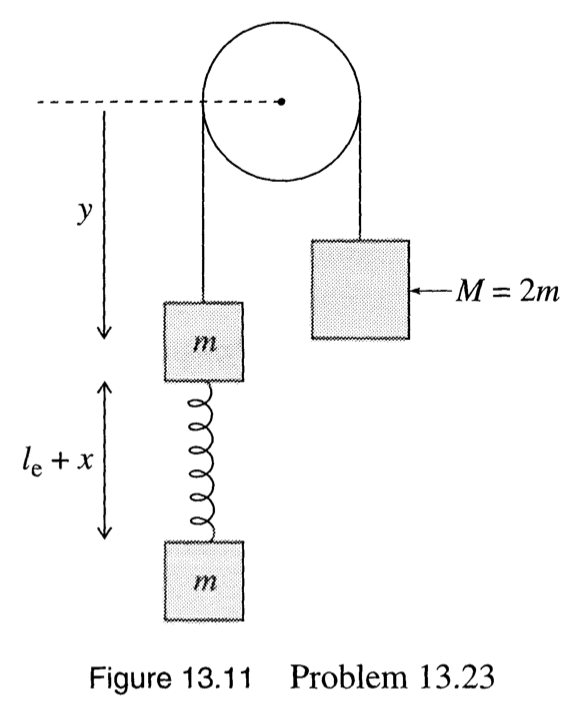
\includegraphics[scale=0.7]{atwood}\]

\begin{enumerate}[(a)]
\item Show that the total potential energy (spring plus gravitational) is just $U = \half k x^2$ (plus a constant that we can take to be zero).

\item Find the two momenta conjugate to $x$ and $y$. Solve for $\dot x$ and $\dot y$, and write down the Hamiltonian. Show that the coordinate $y$ is ignorable. 

\item Write down the four Hamilton equations and solve them for the following initial conditions: You hold the mass $M$ fixed with the whole system in equilibrium and $y = y_0$. Still holding $M$ fixed, you pull the lower mass $m$ down a distance $x_0$, and at $t = 0$ you let go of both masses. [\textit{Hint}: Write down the initial values of $x$, $y$ and their momenta. You can solve the $x$ equations by combining them into a second-order equation for $x$. Once you know $x(t)$, you can quickly write down the other three variables.] Describe the motion. In particular, find the frequency with which $x$ oscillates.

\end{enumerate}
\end{problem}
\end{problem}
\begin{solution}


\vfill
\end{solution}

\end{document}
